% Turabian Formatting for Research Papers Template, 2018/08/06
%
% Developed using the turabian-formatting package (2018/08/01), available through CTAN: http://www.ctan.org/pkg/turabian-formatting
%
% Additional document class formatting options:
%
% raggedright: ragged right formatting without hyphenations
% authordate: support for the author-date citation style
% endnotes: support for endnotes


\documentclass{turabian-researchpaper}

\usepackage [english]{babel}
\usepackage [autostyle, english = american]{csquotes}
% \MakeOuterQuote{"}
% \usepackage[utf8]{inputenc}
% \usepackage{csquotes, ellipsis}

% Specify paper size with geometry package
\usepackage[pass, letterpaper]{geometry}

% For citations, use the biblatex-chicago package
% \usepackage{biblatex-chicago}
% \addbibresource{works-cited.bib}
% \usepackage[sorting=none]{biblatex}
\usepackage{natbib}
\bibliographystyle{abbrv}

% Information for title page
\title{Evaluating Software Technologies}
\subtitle{A deep look into MVC, Event Sourcing, and Database-per-Service}
\author{Layla Arab}
\course{SENG 401}
\date{\today}


\begin{document}

\maketitle


\section{Striving for Functionality}

\begin{quotation}
\begin{tabular}{|p{15cm}}
     "Architecture is about the important stuff. Whatever that is."  - Ralph Johnson\cite{fowler}
\end{tabular}
\end{quotation}

\paragraph{}
While Ralph Johnson’s comment may sound simplistic, it carries a lot of meaning. The architecture of a system provides a basis of communication.\cite{nirmalya_karam_mohsin_2018} This extends to a lot more than just developer communication. System architecture is primordial for the understanding, negotiation, and communication between all the stakeholders.
\par
\paragraph{}
Our current development model faces issues pertaining to the design of our system. This paper will propose several different technologies to integrate into our system. The technology must be capable of solving a current issue with our system to be worth implementing. The purpose of each technology and the method in which it could be integrated into our system will be discussed. The most important metrics of technology will also be outlined.
\par
\paragraph{}
We will firstly assess the scalability of each technology. In this context, scalability is the ability of the system to grow and manage increased demand. \cite{techopedia.com} Scalability alludes to stability and productivity. As such, it is an important metric to consider.
\par
\paragraph{}
Software testability is the degree to which a system supports testing. High testability indicates ease of finding defects in the system through testing methods.\cite{wikipedia_2019}
This is particularly important at scale, considering that it takes a lot of manpower and time to test a large system manually. The time invested by testers must be effective in preventing system faults.
\par
\paragraph{}
Data consistency is another factor to consider. 
Data consistency means that there is conformity in the measurement of variables throughout the datasets.\cite{wikipedia_2018}
Data is one of the most important tools at a business’ disposal.\cite{import.io_2019} Inconsistent data can lead to misinformed data decisions. 
\par
\paragraph{}
The system must be designed on account of the fact that developers work in a team. A complex system that is able to be broken up into modules is ideal for a team following an agile methodology. If a system is unable to be broken down, it becomes unnecessarily complex to develop upon.
\par
\endsection

\clearpage
\section{Model-View-Controller (MVC) Architecture}
\begin{wrapfigure}[13]{L}{0.25\textwidth}
\centering
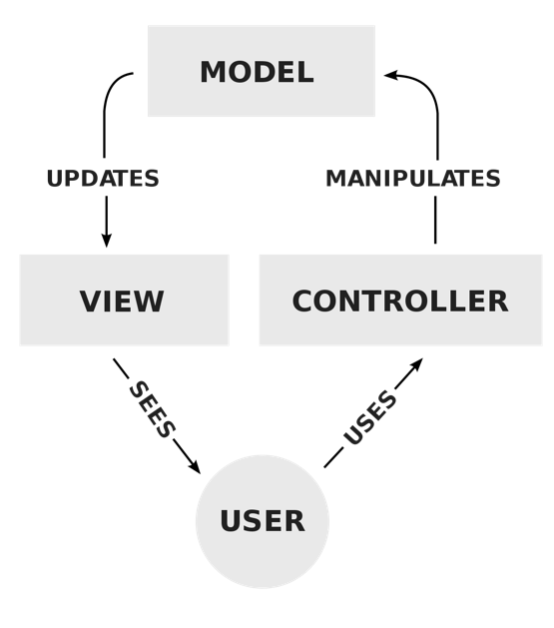
\includegraphics[width=0.25\textwidth]{pics/mvc.png}
\caption{Model-View-Controller Architecture}\cite{wikipedia_2020}
\end{wrapfigure}
\paragraph{}
Model-View-Controller (MVC) Architecture
Due to its versatility, the MVC design pattern is one of the most recognizable software architectures. It helps developers in writing write better organized, and therefore more maintainable code. This pattern has been used and extensively tested over multiple languages and generations of programmers. \cite{chrome}
\par
\paragraph{}
The MVC design pattern is commonly used for developing user interfaces which divide the program logic into modules.
\cite{wikipedia_2020}
Its rising popularity in web application design has lead to the rise of many recognizable frameworks that are used for web development “straight out of the box.” \cite{microsoft}
\par
\paragraph{}
The MVC architecture is made up of the following three interconnected components:\cite{mdnwebdocs}
\par
\paragraph{Model}
Being the central, core component of the pattern,\cite{wikipedia_2020} it is the application's dynamic data structure, as well as its logic and the rules. Through manipulating these attributes, it can present data to the user in the way in which the requirements intend.\cite{UnitTesting} The model does not know anything about the view and controller components. \cite{microsoft}
\par
\paragraph{View}
Forming the user-friendly interface, this is the component presented to the users and dictates how users interact with the app. The view obtains its information from the model; however, the MVC architecture does not allow the view to directly retrieve or update data in the model. \cite{wikipedia_2020}\cite{mdnwebdocs} It must communicate this through controllers.
\paragraph{Controller}
Accepts input and converts it to commands for the model or view. It is responsible for being the decision-maker component by updating the model and the view when they are altered.\cite{wikipedia_2020} More concisely, it is the glue between the model and the view.\cite{chrome}
\par
\subsection{How is this applicable to our application?}
The MVC design is surely popular, but why choose this design pattern over many others? For our company, in particular, the MVC pattern is effective for the reasons discussed below.
\paragraph{}
Simultaneous development is one of our company’s greatest challenges. Our current code is not modular, merges frequently have conflicts. With MVC, multiple developers can work simultaneously on the application due to the inherent modularity of the architecture.\cite{UnitTesting}  
\par
\paragraph{}
MVC boasts being one of the most cohesive and uncoupled architectures.\cite{wikipedia_2020} For this reason, programs with architectures that follow the MVC pattern are scalable. The pattern provides a predictable design for developers, thus enhancing the maintainability and organization. Implementing this architecture gives our application room to grow.
\par
\paragraph{}
Our testers’ productivity can be improved. The modularity drives the code to become better suited for testing in the unit testing context. Bugs become more easy to locate due to the abstractable nature of the pattern. 
\cite{UnitTesting}\cite{wikipedia_2020}
\par
\endsubsection
\endsection


\section{Database-per-service}
\begin{wrapfigure}[15]{L}{0.34\textwidth}
\centering
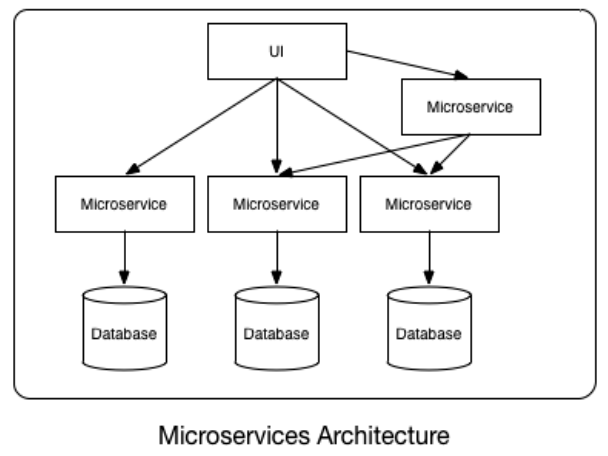
\includegraphics[width=0.35\textwidth]{pics/db.png}
\caption{Database-per-Service Architecture}\cite{mjaglan.github.io}
\end{wrapfigure}
\paragraph{}
Software architecture is important. But it is far from being the only factor that must be considered. Proper database design is integral to a system. At its heart, modern web development is database driven.
\cite{sullivan}\cite{plainoldobjects_2015}
\par
\paragraph{}
Microservice architecture is on the rise. While we will not be talking about microservices in this paper, it is a deeply useful pattern for modularizing applications. Layouts of databases must change in response to this, they must be modularized to match.\cite{microservices.io}
\par
\paragraph{}
The database per service pattern requires that services are loosely coupled, and that there exists a database for every different service. Each service’s persistent data should be kept private, accessible only by its API. This prevents another service from mistakenly making API calls to another service’s database.\cite{microservices.io}
\par
\subsection{How is this applicable to our application?}
\paragraph{}
Database-per-service allows changes to be made to one service’s database without affecting any other services. In addition to this, splitting up databases simplifies them. This makes additions to databases simpler, enforcing data consistency.\cite{microservices.io}
\par
\paragraph{}
We have long had complaints about our page refresh times being too slow. A major factor to this is heavy load our database undergoes constantly. The application cannot access the database fast enough to be acceptable by the users. Splitting our single database into multiple parallelises database accesses, significantly speeding up querying.
\paragraph{}
The database-per-service pattern is fully scalable. More databases can be added as more services are added, keeping up with the growth of the application. 
\par
\endsubsection
\endsection

\section{Event Sourcing}
\paragraph{}
After taking a deep look into database architecture, we need to decide how to persist data into it. Databases need to be updated reliably and automatically. Event sourcing is the perfect tool to achieve this.\cite{microservices.io}
\par
\paragraph{}
Every process can be modelled as a sequence of events. Event-sourcing can be modeled as a normal conversation. Since this is so deeply intuitive, it is easy to build a system exactly as described by a client using this technology.\cite{sullivan}Event-sourcing focuses on the state of the entity. It continuously persists the entity’s state-changing events.\cite{microservices.io}
\par
\subsection{How is this applicable to our application?}
\paragraph{}
Our databases are currently under too much load. Event sourcing speeds up querying speeds, improving load. It continuously stores the activity of the user in the background, having it ready for querying before it is asked for. The results produced are perfect for caching. Webpages can then load more quickly since less data has to be queried. Additionally, since databases are optimized for append only operations, storing data is fast. Events, being append only, are perfectly suited for database integration.\cite{sullivan}
This by default leads to faster refresh times, another aspect our application has struggled with.
\par
\paragraph{}
Event sourcing focuses on states of entities. Because of this, it can be extended to include the state of any additional entity added to the application. Event sourcing is therefore fully scalable. This focus on small changes to an application makes it easier to modify data in a consistent manner, enforcing data consistency.\cite{microservices.io}
\par
\paragraph{}
Event sourcing requires developers to write shorter methods as every event needs its own way in which to query data. This is a change our developers will need to be aware of if we decide to move forward with implementing this design pattern. Shorter methods also tend to be easier to test, making our team more efficient moving forward.\cite{hauer_2019}
\par
\endsubsection
\endsection

\clearpage
\section{A Cohesiveness Assessment}
\paragraph{}
It is important that the suggested architectures are compatible to maintain application balance. The best stacks are those that complement each other, while still being modular and uncoupled.\cite{nirmalya_karam_mohsin_2018}
\par
\paragraph{}
Since database-per-service is a huge change to the architecture of the company’s database, it would be very useful to build a back-end that is flexible when it comes to the tool and structure of database used. This is why event sourcing is perfect to use with database-per-service. It is flexible and gives room for change.
\cite{sullivan}
\par
\paragraph{}
The MVC architecture provides a basis on which design patterns can live. It is a good starting point for any web application due to its versatility. The addition of event sourcing and database-per-service would be seamless if MVC is decided to be integrated into our application. 
\par
\paragraph{}
Event sourcing would exist in the controller of our MVC architecture, where it would use custom-made APIs built for each distinctive database in our database-per-service. The event sourcing mechanisms would keep track of changes in the application, making sure to report this to the views and the models. This would enhance the modularity of the application’s code.\cite{wikipedia_2020}
\par
\endsection

\section{Conclusion}
\paragraph{}
Adding new capabilities to poorly designed software is slow and expensive.\cite{fowler} It also limits the ability of the software to grow.\cite{googlesites}
This is why ensuring high internal quality is fundamental to system design. It leads to the faster delivery of new features. This paper focused on bringing modern software architectures to light, possibly integrating them with our current system.
 \par
 \paragraph{}
The stack that was proposed in this paper answers all of the main problems with our current development methodologies. The technologies all had good reviews on the applicable metrics considered in this paper. 
\par
\endsection


\clearpage
\bibliography{works-cited.bib}
% \printbibliography
\end{document}
